\subsection{Análise anual}
Inicialmente, foram levantadas as quantidades de ligações registradas durante o ano e a quantidade total de falhas, assim como o percentual de falhas. No ano de 2021, que contou com 261 dias de trabalho, foram registradas 51.708 ligações, sendo que 4.227 destas demoraram mais de 60 segundos para serem atendidas, caracterizando falha do processo. O percentual destas falhas para o ano foi de 8,17\%, valor que atende as especificações de desempenho da empresa. No entanto, como este valor representa apenas uma média anual, devemos buscar compreender o problema da empresa ao avaliar o comportamento das variáveis relevantes do processo ao longo do ano.

\subsubsection{Quantidade de chamados por dia}
A Figura \ref*{fig: chamados-tempo} apresenta a quantidade de chamadas recebidas por dia ao longo do ano. É possível perceber uma relação de dependência entre a quantidade de ligações recebidas e os dias do ano, visto que o número de chamadas cresce ao longo do ano. Esse comportamento pode ser responsável pelo aumento do percentual de falhas em meses próximos ao fim do ano. Posteriormente, será descrito um estudo de regressão para estes dados.

\begin{figure}[H]
    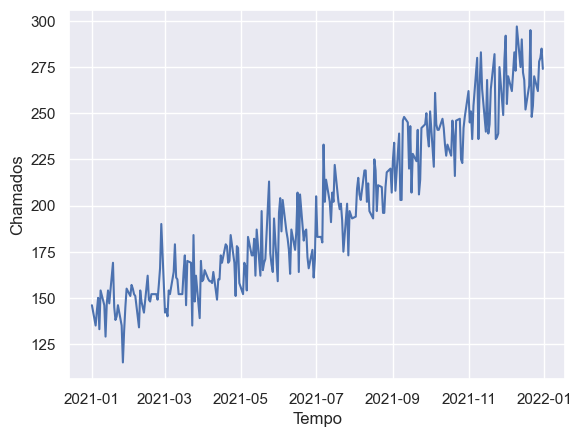
\includegraphics{analise-de-dados/anual/chamados.png}
    \caption{Quantidade de chamadas recebidas ao longo do tempo}
    \label{fig: chamados-tempo}
\end{figure}

\subsubsection{Análise e descrição dos tempos de espera e serviço}
Como os tempos de espera (\textit{wait length}) e serviço (\textit{service length}) já estão calculados, podemos analisar seu comportamento. A Tabela \ref*{tab: descricao-serviço-espera} apresenta as estatística descritivas dos tempos de espera e dos tempos de serviço. É notável que a maioria dos tempos de espera (pelo menos 75\% deles) são nulos, e a média fica abaixo dos 60 segundos, no entanto, o valor máximo é muito elevado. O tempo de serviço também apresenta um valor máximo distante da média.

\begin{table}[H]
\centering
    \begin{tabular}{lr}
        % \begin{center}
            \toprule
            {} &  Tempo de espera \\
            \midrule
            count &   51708.000  \\
            mean  &      17.035  \\
            std   &      64.061  \\
            min   &       0.000  \\
            25\%   &       0.000  \\
            50\%   &       0.000  \\
            75\%   &       0.000  \\
            max   &     983.000  \\
        % \end{center}
        \bottomrule
        % \label{tab: describe-wait}
    \end{tabular}
    \quad
    \begin{tabular}{lr}
        % \begin{center}
            \toprule
            {} &  Tempo de serviço \\
            \midrule
            count &     51708.000   \\
            mean  &       299.103   \\
            std   &       299.866   \\
            min   &         0.000   \\
            25\%   &        86.000   \\
            50\%   &       208.000   \\
            75\%   &       414.000   \\
            max   &      3110.000   \\
        % \end{center}
        \bottomrule
        % \label{tab: describe-wait}
    \end{tabular}
    \caption{Estatística descritiva dos tempos de espera e de serviço}
    \label{tab: descricao-serviço-espera}
\end{table}

Para visualizar a distribuição dos valores estudados, foram criados boxplots. A Figura \ref*{fig: box-wait} mostra o boxplot para a variável de tempos de espera apresentando outliers moderados. A Figura \ref*{fig: box-time} é o boxplot dos tempos de serviço e seus outliers moderados. Em nossa análise, decidimos não retirar os outliers, pois é interessante para o problema a modelagem de variáveis aleatórias com distribuições que levem em consideração a presença de valores extremos (caudas longas).

\begin{figure}[H]
    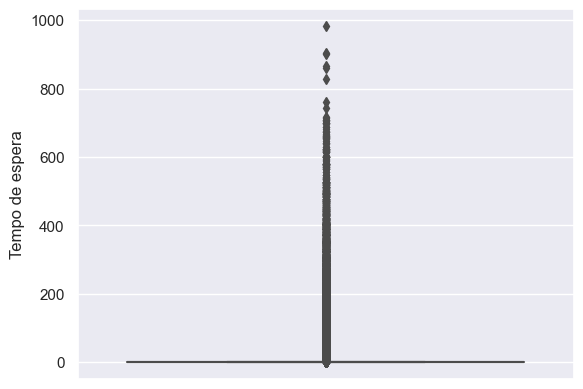
\includegraphics{analise-de-dados/anual/box-wait.png}
    \caption{Boxplot tempos de espera}
    \label{fig: box-wait}
\end{figure}

\begin{figure}[H]
    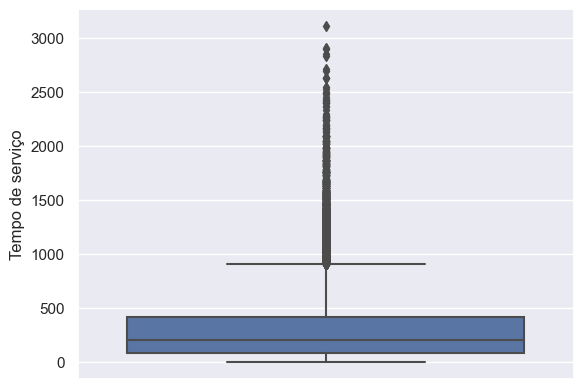
\includegraphics{analise-de-dados/anual/box-service.png}
    \caption{Boxplot tempos de serviço}
    \label{fig: box-time}
\end{figure}

O comportamento do tempo médio de serviço ao longo do ano pode ser visto na Figura \ref*{fig: t_servico-tempo} e apresenta um caráter permanente.

\begin{figure}[H]
    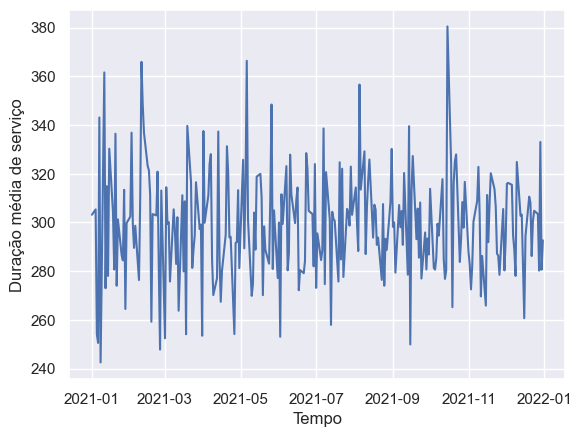
\includegraphics{analise-de-dados/anual/service_len.png}
    \caption{Tempos médios de serviço ao longo do tempo}
    \label{fig: t_servico-tempo}
\end{figure}

Para testar a hipótese que o tempo de serviço segue uma mesma distribuição ao longo do ano, foi utilizado o teste não paramétrico de Kolgomorov-Smirnov com duas amostras, testando os meses dois a dois. Os resultados estão na Figura \ref*{fig: KS_servico}. As células em verde possuem valor $p$ maior que o nível de significância adotado que é $\alpha = 5\%$, e, portanto não há diferenças estatisticamente significativas entre a distribuição dos tempos de serviço ao longo dos meses do ano.

\begin{figure}[H]
    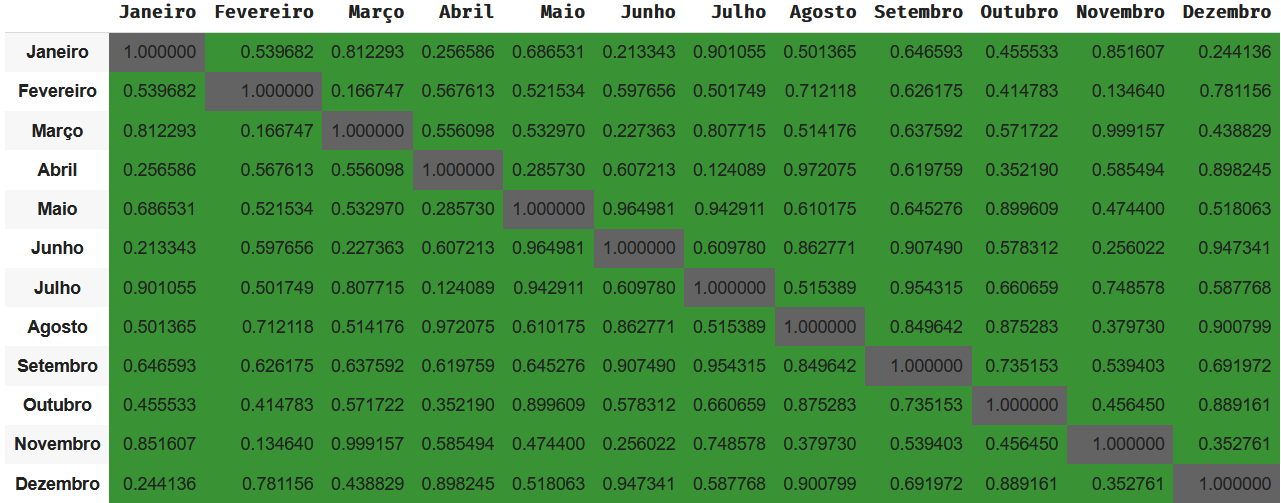
\includegraphics[scale=0.6]{analise-de-dados/anual/ks-service.png}
    \caption{$p$ valores do teste KS 2 amostras para tempos de serviço}
    \label{fig: KS_servico}
\end{figure}

O tempo médio de espera ao longo do ano é representado na Figura \ref*{fig: espera-tempo}. A Figura \ref*{fig: KS_wait} mostra o teste de hipóteses para os tempos de espera mês a mês. É possível concluir que no início do ano (até o mês de maio), não houve diferenças significativas entre os tempos de espera. No entanto, a partir de junho, é possível atestar diferenças mais acentuadas na distribuição dos tempos de espera, representado pelos $p$ valores abaixo de 5\%, apresentado pelas células em vermelho.

\begin{figure}[H]
    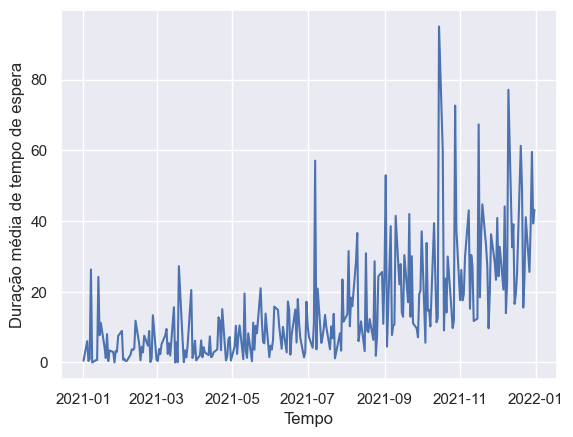
\includegraphics{analise-de-dados/anual/service.png}
    \caption{Tempos médios de espera ao longo do ano}
    \label{fig: espera-tempo}
\end{figure}

\begin{figure}[H]
    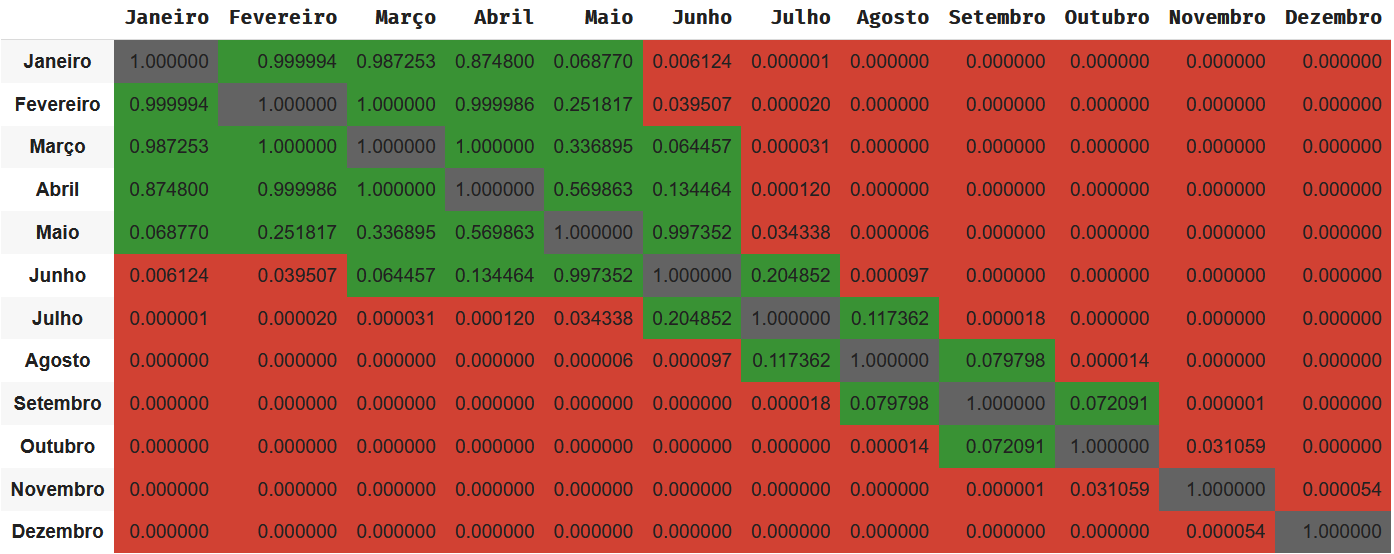
\includegraphics[scale=0.55]{analise-de-dados/anual/ks-wait.png}
    \caption{$p$ valores do teste KS 2 amostras para tempos de espera}
    \label{fig: KS_wait}
\end{figure}

\subsubsection{Fit dos tempos serviços}
